\documentclass[hyperref={pdfpagelabels=false}]{beamer}
%\documentclass[handout]{beamer}
\usepackage[ngerman]{babel}
\usepackage{amsmath}
\usepackage{amsfonts}
\usepackage{amssymb}
\usefonttheme{serif}
\usepackage[utf8]{inputenc}
\usepackage {graphicx}
\usepackage [T1]{fontenc}
\usepackage{listings} %Quellcode mit \lstinline{} oder mit \begin ... darstellen
\usepackage{hyperref}
\usepackage{fancyvrb}

\usepackage{siunitx}

\usepackage{caption}
\usepackage{subcaption}
\captionsetup[subfigure]{labelformat=empty}

% TikZ
%\usepackage[landscape]{geometry}
\usepackage{tikz}
\usetikzlibrary{mindmap}
\usepackage{metalogo}
\usepackage{dtklogos}
\usepackage{adjustbox}

\usepackage{bbding}
\usepackage{overpic}

%\pgfpagesuselayout{4 on 1 with notes}[a4paper,border shrink=5mm]
\title[\LaTeX-Einführung]{\LaTeX-Kurs}
\institute[]{Fachschaft Physik, Uni Frankfurt}
\author[Marco, Ben]{Marco Knipfer \\ Ben Arnoldi-Meadows}
%\usetheme{Warsaw}
\date{Freitag, 13.04.18}
\usetheme{Madrid}
%\usecolortheme{default}
\beamertemplatenavigationsymbolsempty
\providecommand{\thispdfpagelabel}[1]{}


\begin{document} 
\begin{frame}[plain]
    \maketitle
\end{frame}
\begin{frame}[plain]
    \tableofcontents
\end{frame}
\section{Um was geht es heute?}
\begin{frame}{Der \LaTeX{}-Kurs}
    \begin{block}{Um was geht es heute? - die Themen}
        \begin{itemize}
            \item Was ist \LaTeX{}, wieso \LaTeX{}? Einführung und Installation
            \item Gemeinsames Erstellen eines Praktikumprotokolls
                \begin{itemize}
                    \item Theorie hier am Beamer
                    \item Anwendung im Protokoll
                \end{itemize}
        \end{itemize}
    \end{block}
\end{frame}

\section{Was ist \LaTeX{}?}

\begin{frame}{Was ist \LaTeX{}?}
    \begin{block}{?? \TeX{}, \LaTeX{}??}
        \begin{itemize}
            \item Textsatzprogramm\\
            \LaTeX{}=Buch-Designer, \TeX{}=Setzer
            \item Ideale Organisation umfangreicher Dokumente
            \item Kein WYSIWYG!
        \end{itemize}
    \end{block}
\end{frame}
\begin{frame}{Wozu ist \LaTeX{} NICHT?}
    \begin{block}{Nicht für}
        \begin{itemize}
            \item Tabellenkalkulation
            \item Multimedia-Shows
            \item Darstellung von Messwerten, Plots
            \item Plakate nur bedingt
        \end{itemize}
    \end{block}
\end{frame}
\begin{frame}{Wozu dann?}
    \begin{block}{Gute Argumente}
        \begin{itemize}
            \item Einfache Formatierung
            \item Mathematische Formeln sehr elegant und einfach
            \item Wirkt sehr professionel
            \item OpenSource
            \item Plattformunabhängig
        \end{itemize}
    \end{block}
\end{frame}
\begin{frame}{Installation von \LaTeX{}}
    \begin{block}{Plattformen}
        \begin{itemize}
            \item Windows, Unix: TeX Live \url{http://www.tug.org/texlive/}
            \item Mac: MacTex \url{http://www.tug.org/mactex/}
        \end{itemize}
    \end{block}
    \begin{block}{\LaTeX{}-Editor}
        \begin{itemize}
            \item Texteingabe, Bearbeitung, Syntax-Hervorherbung, Shortcuts
            \item Wir empfehlen: \textit{Texmaker} für alle Plattformen
            \item Auch gut um zu zweit Protokolle zu schreiben: \textit{ShareLaTeX}
            \item Für Nerds: VIM + LaTeX-Suite
        \end{itemize}
    \end{block}
\end{frame}
\begin{frame}[plain]
    \includegraphics[width=\textwidth]{pics/texmaker.png}
\end{frame}
\begin{frame}[plain]
    \includegraphics[width=\textwidth]{pics/sharelatex.pdf}
\end{frame}
\begin{frame}[plain]
    \includegraphics[width=\textwidth]{pics/vim.pdf}
\end{frame}

\section{\LaTeX{}-Grundlagen}

\begin{frame}[fragile]{\LaTeX{}-Grundlagen}
    \begin{block}{Wichtiges zuerst!}
        Zwei essentielle Dinge werden getrennt!
        \begin{itemize}
            \item Verfassen des Inhalts
            \item Darstellung / Formatierung
        \end{itemize}
    \end{block}
    \pause
    \begin{block}{Befehle}
        \begin{itemize}
            \item Beginnen immer mit Backslash \verb!\!
            \item Unterscheidung:\\
                \verb!\befehl{Angabe1}{Angabe2}{Angabe3}!\\
                \verb!\befehl 123!
        \end{itemize}
    \end{block}
\end{frame}

\begin{frame}[fragile]{Dokumentstruktur}
\begin{Verbatim}
HEADER (Präambel)

\begin{document}

BODY

\end{document}
\end{Verbatim}
\end{frame}
    
\begin{frame}[fragile]{Der Header - Der Kopf}
    \begin{block}{Der Header - Der Kopf}
        Globale Informationen zum Dokument\\
        \begin{description}
            \item[Klasse] \verb!\documentclass[Optionen]{Klasse}!\\
                KOMA-Skript Klassen: scrartcl, scrbook
            \item[Packages] \verb!\usepackage{package}!\\
                babel, amsmath, \dots
            \item[Titel] Wird z.B. beim Befehl \verb!\maketitle! genutzt:\\
                \verb!\title{Dokumnttitel}!\\
                \verb!\author{Author}!\\
                \verb!\date{Datum}!
        \end{description}
    \end{block}
\end{frame}
\begin{frame}[fragile]{Beispielheader}
\begin{verbatim}
\documentclass[12pt,a4paper, final]{scrartcl}
\usepackage[ngerman]{babel} % Deutsche Sprachanpassungen
\usepackage[utf8]{inputenc} % Direkte Angabe von Umlauten
\usepackage[T1]{fontenc}

\usepackage{amsmath}  % Mathe
\usepackage{hyperref} % Links
\usepackage{graphicx} % Z.B. .jpg Bilder einbinden
\end{verbatim}
\end{frame}

    
\section{Bau unseres Praktikumprotokolls}
\subsection{Hello World}
\begin{frame}[fragile]{Hello World}
    Anfang mit Protokoll $\rightarrow$ ihr habt das Ausgedruckte "`Musterprotokoll"'
    \pause
    \begin{block}{Erstes Dokument - Hello World}
        \begin{Verbatim}[frame=single]
\documentclass{scrartcl}
% Dies ist ein Kommentar
\begin{document} % hier beginnt das Dokument
Hello World!
\end{document}
        \end{Verbatim}
    \end{block}
    \pause
    Probiert es aus!
\end{frame}

\subsection{Titelseite}
\begin{frame}[fragile]{Die Titelseite}
    \includegraphics[width = \textwidth]{pics/Anfang-Protokoll.pdf}
\end{frame}

\subsection{Strukturierung unseres Protokolls}
\begin{frame}[fragile]{Strukturierung unseres Protokolls}
    \begin{block}{Strukturierung}
        \begin{Verbatim}
\section{Geschichte des Glücksspiels}
    \subsection{Einführung}
    \subsection{Der Würfel}
\section{Versuchsaufbau und Ergebnisse}
        \end{Verbatim}
    \end{block}
    \pause
    Bei manchen Klassen (book) gibt es noch über sections \verb!\chapter{}!.
\end{frame}

\begin{frame}[fragile]{Das Inhaltsverzeichnis}
    \begin{block}{TOC Table of Contents}
        \begin{itemize}
            \item \verb!\tableofcontents!
            \item Info wird in .toc Datei gespeichert
            \item Erst beim nächsten Kompilieren vorhanden
            \item Manche Sachen stimmen dann auch erst beim 3. Kompilieren (z.B.
                Angabe der Seitenzahlen im TOC)
                \pause
            \item \verb!\listoftables! \verb!\listoffigures!
            \item Literaturverzeichnis später
        \end{itemize}
    \end{block}
\end{frame}
\begin{frame}[fragile]{Text}
    \begin{block}{Text?}
        \begin{itemize}
            \item Einfach schreiben! =)
            \item Sonderzeichen? $\rightarrow$ backslash davor (meistens)
            \item \& $\rightarrow$ \verb!\&!
            \item \{\} $\rightarrow$ \verb!\{\}!
            \item \$ $\rightarrow$ \verb!\$!
            \item \% $\rightarrow$ \verb!\%!
        \end{itemize}
    \end{block}
    \pause
    AUSPROBIEREN!
    \begin{Verbatim}[frame=single]
    \subsection{Einführung}
    Hier schreibe ich ein Wenig Text!
    \end{Verbatim}
\end{frame}

\begin{frame}[fragile]{Code-Formatierung?}
    \begin{block}{\LaTeX{}-Code Formatierung}
        \begin{itemize}
            \item Neue Zeilen werden ignoriert
            \item[$\rightarrow$] wirkliche neue Zeile \verb!\\!
                oder \verb!\newline!
            \item Leerzeile $\rightarrow$ neuer Paragraph (indent)
                \pause
            \item Empfehlung: Schreibt keine zu langen Zeilen,
                lieber neue Zeile anfangen (übersichtlicher!).
                \pause
            \item Meine Praxis: Nach jedem Satzende neue Zeile,
                Codeblöcke einrücken.
        \end{itemize}
    \end{block}
    \pause
    \footnotesize
    \begin{Verbatim}
\begin{itemize}
    \item banana
    \item
        \begin{enumerate}
            \item bla
            \item blup
        \end{enumerate}
\end{itemize}
    \end{Verbatim}
\end{frame}

\subsection{Itemize}
\begin{frame}[fragile]{Auflistungen}
    \begin{block}{itemize}
        \begin{itemize}
            \item Aufzählung, so wie hier
                \begin{Verbatim}
\begin{itemize}
    \item Erster Punkt
    \item Zweiter Punkt
\end{itemize}
                \end{Verbatim}
                \pause
            \item \verb!\item[$\rightarrow$]!
            \item[$\rightarrow$] Pfeil
        \end{itemize}
    \end{block}
    \pause
    \begin{block}{enumerate}
        \begin{enumerate}
            \item Aufzählung
                \pause
            \item kann auch geschachtelt werden
                \pause
                \begin{itemize}
                    \item So
                    \item wie
                    \item hier
                \end{itemize}
        \end{enumerate}
    \end{block}
\end{frame}

\begin{frame}[fragile]{Description}
    \begin{block}{description}
        \begin{description}
            \item[Faust]
                Habe nun, ach! Philosophie, \\
                Juristerei und Medizin, \\
                Und leider auch Theologie \\
                Durchaus studiert, mit heißem Bemühn. \\
                Da steh ich nun, ich armer Tor!
            \item[Geist] Wer ruft mir?\\
        \end{description}
    \end{block}
    \pause
    \begin{block}{}
        \begin{Verbatim}
\begin{description}
    \item[Faust:]
        Habe nun, ach! Philosophie, \\
        . . . 
        Da steh ich nun, ich armer Tor!
    \item[Geist] Wer ruft mir?\\
\end{description}
        \end{Verbatim}
    \end{block}
\end{frame}

\subsection{Textanpassungen}
\begin{frame}[fragile]{Textanpassungen}
    \begin{block}{Textanpassungen}
            \begin{itemize}
                \item Textgrößen: \verb!\begin{tiny} blabla \end{tiny}! oder
                    \verb!\tiny!
                \item tiny, scriptsize, footnotesize, small, normalsize, large,
                    Large, LARGE, huge, Huge
                    \pause
                \item \verb!\textbf{fetter Text}!: \textbf{fett}
                \item \verb!\underline{unterstrichener Text}!: \underline{unterstrichen}
                \item \verb!\textit{kursiver Text}! (italic): \textit{italian}
                \item \verb!\emph{betont}!: \emph{betont}
                \item \verb!\textsc{kapitälchen}!: \textsc{Das sind Kapitälchen}
            \end{itemize}
    \end{block}
\end{frame}

\subsection{Einfügen von Bildern}
\begin{frame}[fragile]{Einfügen von Bildern}
    \begin{block}{Bilder}
        \begin{itemize}
            \item \verb!\usepackage{graphicx}!
            \item Float Umgebung \verb!\begin{figure}!
            \item Zentrieren mit \verb!\centering!
            \item Bild einfügen mit \\
                \verb!\includegraphics[width=0.5\textwidth]{figures/dice.jpg}!
            \item Bildunterschrift mit \verb!\caption{Unterschrift}!
            \item Internes Label mit \verb!\label{fig:wuerfel}!
        \end{itemize}
    \end{block}
\end{frame}

\begin{frame}[fragile]{Bilder - Code}
    \begin{Verbatim}[frame=single]
\begin{figure}[h] % h here, t top, b bottom
    \centering
    \includegraphics[width=0.5\textwidth]{figures/dice.jpg}
    \caption{Klassische Spielwürfel (aus \cite{wiki:wuerfel}, wie man
    solche Quellenangaben macht lernt ihr später!)}
    \label{fig:wuerfel}
\end{figure}
    \end{Verbatim}
\pause
Package \verb!float! für Option \verb!H! (genau hier)
\end{frame}
\begin{frame}{Bilder - Ergebnis}
    \includegraphics[width=\textwidth]{pics/bilder.pdf}
\end{frame}

\begin{frame}[fragile]{Mehrere Bilder in einer Float - subfigure}
        \footnotesize
        \begin{Verbatim}
\usepackage{subcaption}

\begin{figure}
    \centering
    \begin{subfigure}[b]{0.49\textwidth}
        \includegraphics[width=\textwidth]{fig1}
        \caption{caption1}
        \label{fig:label1}
    \end{subfigure}
    \hfill
    \begin{subfigure}[b]{0.49\textwidth}
        \includegraphics[width=\textwidth]{fig2}
        \caption{caption2}
        \label{fig:label2}
    \end{subfigure}
    \caption{Gesamt Caption}
    \label{GesamtLabel}
\end{figure}
        \end{Verbatim}
\end{frame}
\begin{frame}[fragile]{Mehrere Bilder in einer Float - subfigure}
    \begin{figure}
        \begin{subfigure}[b]{0.4\textwidth}
            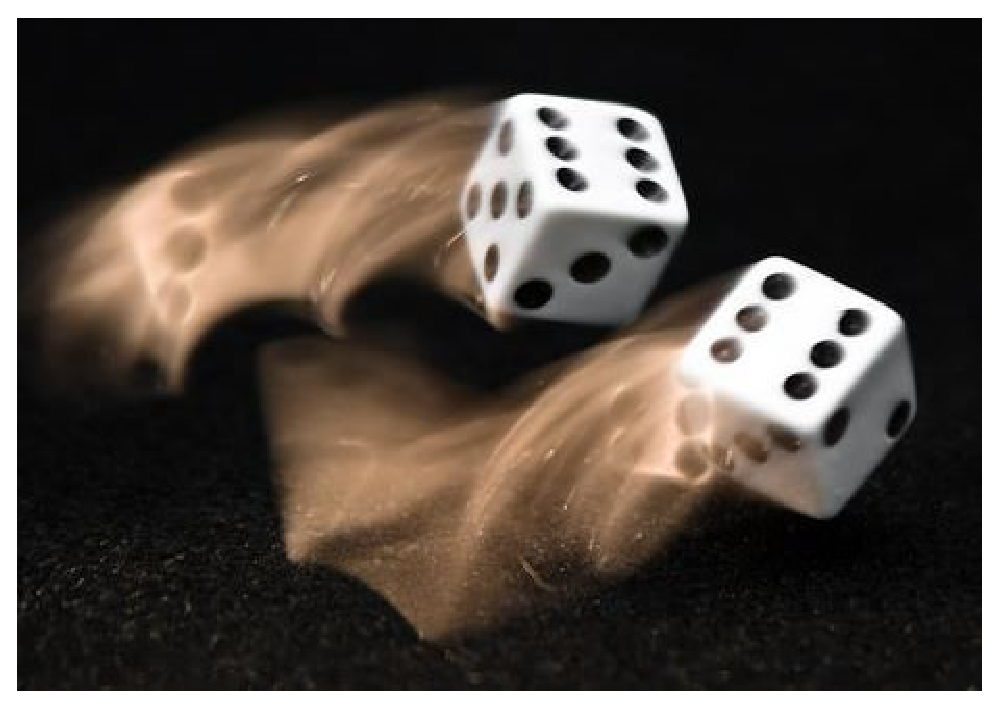
\includegraphics[width=\textwidth]{pics/bildwuerfel1}
            \caption{caption1}
            \label{fig:label1}
        \end{subfigure}
        \hfill
        \begin{subfigure}[b]{0.4\textwidth}
            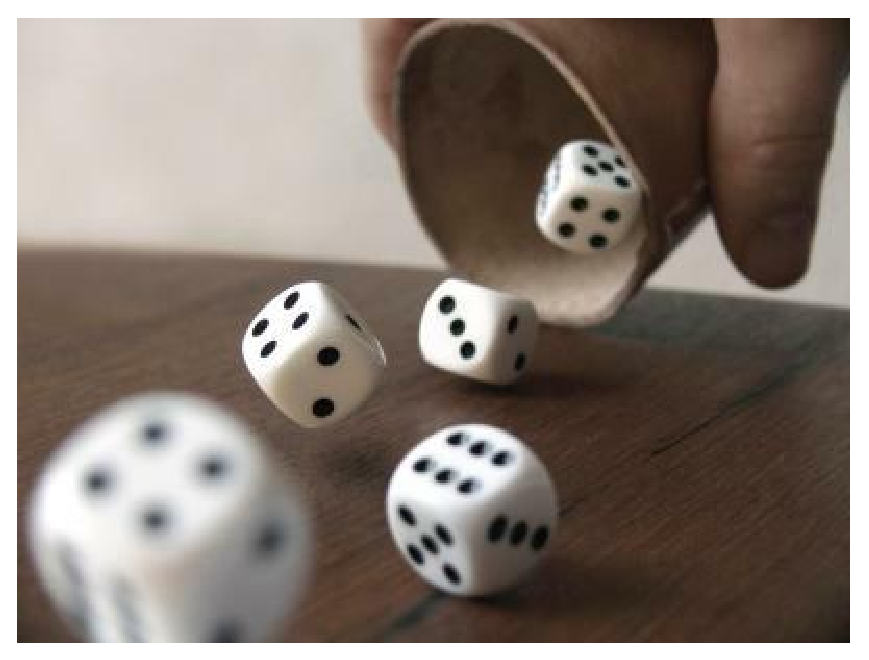
\includegraphics[width=\textwidth]{pics/bildwuerfel2}
            \caption{caption1}
            \label{fig:label2}
        \end{subfigure}
        \caption{Gesamtbild-Unterschrift}
    \end{figure}
\pause
\footnotesize
Packages \verb!subfigure! und \verb!subfig! deprecated, evtl.\ aber noch
für Vorlagen (von Springer o.Ä.) gebraucht
\url{https://en.wikibooks.org/wiki/LaTeX/Floats,_Figures_and_Captions}.
\end{frame}

\subsection{Tabellen}
\begin{frame}{Tabellen}
\begin{table}[h]
    \centering
    \begin{tabular}{c|l|l}
        Zahl & Anzahl & Anteil\\
        \hline
        1 & 100 & 1/6\\
        2 & 102 & 0,17\\ 
        3 & 99 & 0,165\\
        4 & 100 & 1/6\\
        5 & 98 & $0,16\overline{3}$\\
        6 & 101 & $0,168\overline{3}$ 
    \end{tabular}
    \caption{Ergebnisse von 600 Würfen}
\end{table}
\end{frame}

\begin{frame}[fragile]{Tabellen}
    \begin{block}{Tabellen}
        \begin{itemize}
            \item float Umgebung \verb!\begin{table}!
            \item Tabellen Umgebung \verb!\begin{tabular}{<<spalten>>}!
                \item c: center, l: linksbündig (l, nicht 1), r: rechtsbündig
                \pause
            \item |: vertikale Linie
                \pause
            \item nächste Spalte mit \verb!&!
            \item nächste Zeile mit \verb!\\!
            \item horizontale linie mit \verb!\hline!
                \pause
            \item z.B. SciDavis (wie Origin) kann direkt Tabellen als 
                \LaTeX{} Code exportieren
        \end{itemize}
    \end{block}
\end{frame}
\begin{frame}[fragile]{Tabellen - Code}
    \begin{minipage}{0.29\textwidth}
        \begin{table}[h]
            \centering
            \begin{tabular}{c|l|l}
                Zahl & Anzahl & Anteil\\
                \hline
                1 & 100 & 1/6\\
                2 & 102 & 0,17\\ 
                3 & 99 & 0,165\\
                4 & 100 & 1/6\\
                5 & 98 & $0,16\overline{3}$\\
                6 & 101 & $0,168\overline{3}$ 
            \end{tabular}
            \caption{Ergebnisse von 600 Würfen}
        \end{table}
    \end{minipage}
    \hfill
    \begin{minipage}{0.66\textwidth}
        \begin{Verbatim}
\begin{table}[h]
    \centering
    \begin{tabular}{c|l|l}
        Zahl & Anzahl & Anteil\\
        \hline
        1 & 100 & 1/6\\
        2 & 102 & 0,17\\ 
        3 & 99  & 0,165\\
        4 & 100 & 1/6\\
        5 & 98  & 0,16$\overline{3}$\\
        6 & 101 & 0,168$\overline{3}$ 
    \end{tabular}
    \caption{Ergebnisse von 600 Würfen}
\end{table}
        \end{Verbatim}
    \end{minipage}
\end{frame}

\begin{frame}[fragile]{Tabellen anpassen}
Um die Spaltenbreite festzulegen verwendet man als Format
\verb!p{Breite}!
\begin{block}{}
    \begin{Verbatim}
\begin{tabular}{p{5cm}|p{3cm}}
    5 cm breite Spalte   &   3 cm breite Spalte \\
    \hline
    Dies ist eine Spalte, die 5cm breit ist.
    Somit wird Text nach 5cm umgebrochen,
    und die Zellenhöhe angepasst. &
    Diese Spalte ist nur 3cm breit, der Text 
    wird demnach eher umgebrochen. 
    Bei gleicher Textlänge wird die Zelle also höher!
\end{tabular}
    \end{Verbatim}
\end{block}
\end{frame}

\begin{frame}{Tabellen anpassen}
    \begin{block}{Ausgabe}
        \begin{tabular}{p{5cm}|p{3cm}}
            5 cm breite Spalte   &   3 cm breite Spalte \\
            \hline
            Dies ist eine Spalte, die 5cm breit ist.
            Somit wird Text nach 5cm umgebrochen,
            und die Zellenhöhe angepasst. &
            Diese Spalte ist nur 3cm breit, der Text wird demnach eher umgebrochen. Bei
            gleicher Textlänge wird die Zelle also höher!
        \end{tabular}
    \end{block}

\end{frame}

\subsection{Mathematische Ausdrücke}
\begin{frame}[fragile]{$\phi \quad \Phi \quad \varphi \quad$ Mathe \quad $ \Xi \quad \xi \quad \Omega  \quad \zeta$}
    \begin{block}{Mathe Umgebung}
        \begin{itemize}
            \item amsmath Paket verwenden \AmS-\LaTeX\\
                American Mathematical Society
                \pause
            \item Eingerückte Gleichung \verb!\begin{equation}!
                \begin{equation}
                    a^2 + b^2 = c^2
                    \label{eq:pythagoras}
                \end{equation}
            \item (keine Nummerierung \verb!equation*!)
            \pause
            \item inline Gleichung \verb!$gleichung$!\\
                Der Satz des Pythagoras $a^2 + b^2 = c^2$ \dots
        \end{itemize}
    \end{block}
\end{frame}
\begin{frame}[fragile]{Mathe - Die Syntax}
    \begin{block}{Mathesyntax}
        \begin{itemize}
            \item Ziemlich intuitiv
            \item $a^2$ = \verb!a^2!
            \item[$\rightarrow$] Lasst uns ein Paar Beispiele machen
        \end{itemize}
    \end{block}
    \pause
    \begin{equation}
        B(k | p,n) = \binom {n}{k} p^k (1-p)^{n-k}\quad \text{für}\quad k=0,1,\dots, n\,.
        \label{eq:binomial}
    \end{equation}
    \pause
    \begin{Verbatim}
\begin{equation}
    B(k | p,n) = \binom{n}{k} p^k (1-p)^{n-k}\quad 
                 \text{für}\quad k=0,1,\dots, n\,.
    \label{eq:binomial}
\end{equation}
    \end{Verbatim}
    \pause
    Label intern für euch. Verweis auf Glg (\ref{eq:binomial}) mit
    \verb!(\ref{eq:binomial})!
\end{frame}

\begin{frame}[fragile]{Mehrzeilig, Summen, Integrale}
    \begin{minipage}{0.4\textwidth}
        \begin{footnotesize}
            \begin{align}
                \mu &= \sum_{k=0}^n k \binom nk p^k (1-p)^{n-k}\\
                    &= \dots \nonumber\\
                    &= np\quad.
                \label{eq:erwartungswert}
            \end{align}
        \end{footnotesize}
    \end{minipage}
    \hfill
    \begin{minipage}{0.59\textwidth}
        \begin{footnotesize}
        \begin{Verbatim}
\begin{align}
    \mu &= \sum_{k=0}^n k \binom nk p^k (1-p)^{n-k}\\
        &= \dots \nonumber\\
        &= np\quad.
    \label{eq:erwartungswert}
\end{align}
        \end{Verbatim}
        \end{footnotesize}
    \end{minipage}
    ~\\
    ~\\
    \pause
    \begin{minipage}{0.4\textwidth}
        \begin{footnotesize}
            \begin{equation}
                W(\mu, \sigma) = \int_{\mu-j\sigma}^{\mu+j\sigma} P(x,\mu) \mathrm{d}x\quad.
                \label{eq:Standardabweichung}
            \end{equation}
        \end{footnotesize}
    \end{minipage}
    \hfill
    \begin{minipage}{0.59\textwidth}
        \begin{footnotesize}
            \begin{Verbatim}
\begin{equation}
    W(\mu, \sigma) = 
    \int_{\mu-j\sigma}^{\mu+j\sigma} P(x,\mu)
    \mathrm{d}x\quad.
    \label{eq:Standardabweichung}
\end{equation}
            \end{Verbatim}
        \end{footnotesize}
    \end{minipage}
\pause
\\
Wir empfehlen \textsc{kein} \textit{eqnarray} zu benutzen:
\url{https://tug.org/pracjourn/2006-4/madsen/madsen.pdf}\\
\textit{Avoid eqnarray!} von \textit{Lars Madsen}.
\end{frame}
\begin{frame}[fragile]{Weitere Mathe-Befehle}
    Klammern-Größe anpassen:\\
    $\left( \frac{\frac{1}{2} + 1}{3} \right) \neq ( \frac{\frac{1}{2} + 1}{3} )$\\
    \begin{footnotesize}
    \verb!\left(\frac{\frac{1}{2}+1}{3}\right) \neq (\frac{\frac{1}{2}+1}{3})!\\
    \end{footnotesize}
    \pause
    ~ \\
    $\pi \in \mathbb R$ braucht Package amssymb\\
    \verb!\pi \in \mathbb R! \\
    \pause
    ~ \\
    $\mathbf{F}_\text{C} = \frac{1}{4 \pi \epsilon_0}\frac{q_1 q_2}{r^2}\mathbf{\hat{r}}$\\
    \begin{footnotesize}
    \verb!\mathbf{F}_C = \frac{1}{4 \pi \epsilon_0}\frac{q_1 q_2}{r^2}\mathbf{\hat{r}}!
    \end{footnotesize}
    \pause
    ~ \\
    $\vec{v}$\\
    \verb!\vec{v}!
    ~\\~\\
    \pause
    $\underbrace{1 + 2}_3$\\
    \verb!\underbrace{1 + 2}_3!
\end{frame}
\begin{frame}[fragile]{Weiter Mathe}
    \begin{itemize}
        \item Wurzeln: $\sqrt{2}$\\
            \verb!\sqrt{2}!
        \item Optional: $\sqrt[3]{2}$\\
            \verb!\sqrt[3]{2}!
            \pause
        \item Matrizen: Wie Tabellen
            \begin{equation}
                \begin{bmatrix}
                a_1 & a_2 & a_3 & a_4 \\
                b_1 & b_2 & b_3 & b_4 \\
                c_1 & c_2 & c_3 & c_4 \\
                d_1 & d_2 & d_3 & d_4
                \end{bmatrix}
            \end{equation}
            \begin{Verbatim}
\begin{bmatrix}
a_1 & a_2 & a_3 & a_4 \\
b_1 & b_2 & b_3 & b_4 \\
c_1 & c_2 & c_3 & c_4 \\
d_1 & d_2 & d_3 & d_4
\end{bmatrix}
            \end{Verbatim}
    \end{itemize}
\end{frame}
\begin{frame}{Matrizen}
    \begin{itemize}
        \item matrix (nackte Matrix)
        \item bmatrix \{\}
        \item Bmatrix []
        \item pmatrix ()
        \item Vmatrix || ||
        \item vmatrix | |
        \item Bordermatrix
    \end{itemize}
    \pause
    $
    \begin{matrix}
        a_1 & a_2 & a_3 & a_4 \\
        b_1 & b_2 & b_3 & b_4 \\
        c_1 & c_2 & c_3 & c_4 \\
        d_1 & d_2 & d_3 & d_4
    \end{matrix}
    \begin{bmatrix}
        a_1 & a_2 & a_3 & a_4 \\
        b_1 & b_2 & b_3 & b_4 \\
        c_1 & c_2 & c_3 & c_4 \\
        d_1 & d_2 & d_3 & d_4
    \end{bmatrix}
    \begin{Bmatrix}
        a_1 & a_2 & a_3 & a_4 \\
        b_1 & b_2 & b_3 & b_4 \\
        c_1 & c_2 & c_3 & c_4 \\
        d_1 & d_2 & d_3 & d_4
    \end{Bmatrix}
    \begin{pmatrix}
        a_1 & a_2 & a_3 & a_4 \\
        b_1 & b_2 & b_3 & b_4 \\
        c_1 & c_2 & c_3 & c_4 \\
        d_1 & d_2 & d_3 & d_4
    \end{pmatrix}
    $  \\
    $
    \begin{vmatrix}
        a_1 & a_2 & a_3 & a_4 \\
        b_1 & b_2 & b_3 & b_4 \\
        c_1 & c_2 & c_3 & c_4 \\
        d_1 & d_2 & d_3 & d_4
    \end{vmatrix}
    \bordermatrix{
        & 1	& 2   & 3   & 4   \cr
        A & a_1 & a_2 & a_3 & a_4 \cr
        B & b_1 & b_2 & b_3 & b_4 \cr
        C & c_1 & c_2 & c_3 & c_4 \cr
        D & d_1 & d_2 & d_3 & d_4 \cr
    }
    $
\end{frame}
\begin{frame}[fragile]{Punkte in Matrizen}
    \begin{minipage}{0.49\textwidth}
    $
    \begin{bmatrix}
        1       & 0     & \dots  & 0      \\
        0       & 1     & \dots  & 0      \\
        \vdots  & 0     & \ddots & \vdots \\
        0       & \dots & 0      & 1
    \end{bmatrix}
    $
    \end{minipage}
    \begin{minipage}{0.49\textwidth}
        \begin{itemize}
            \item \verb!\dots!
            \item \verb!\vdots! vertikal
            \item \verb!\ddots! diagonal
                \pause
            \item \verb!\cdots! horizontal, aber zentriert
            \item \verb!\cdot! "`Malpunkt"' $2\cdot 10^{42}$
        \end{itemize}
    \end{minipage}
    ~\\~\\
    \begin{Verbatim}
\begin{bmatrix}
    1       & 0     & \dots  & 0      \\
    0       & 1     & \dots  & 0      \\
    \vdots  & 0     & \ddots & \vdots \\
    0       & \dots & 0      & 1
\end{bmatrix}
    \end{Verbatim}
    \pause
    Generelle Empfehlung für Tabellen/Matrizen:\\
    Strukturiert euren Code schön!
\end{frame}

\begin{frame}{Weiter Mathe}
    Wenn ihr lust habt, könnt ihr Mal schauen, wie weit ihr bei diesen Formeln
    kommt (Google!).
    \begin{small}
        \begin{equation}
        \left < q_ft_f | q_it_i \right> = 
        \lim_{n\to \infty} \int \prod_{j=1}^{n} \mbox dq_j 
        \prod_ {j=0}^{n} \frac {\mbox d p_j}{h} 
        \exp \left \{ \frac {i}{\hbar} \sum_{j=0}^{n} 
        \left [ p_j 
        \left( q_{j+1} - q_ {j} \right ) - \tau H \left ( p_j ,\overline{q_j}\right) 
        \right ] \right \}
        \label{eq:path:1}
        \end{equation}
        \begin{equation}
        K_0 = \lim_{n \to \infty} \left ( \frac m {ih\tau} \right) ^{(n+1)/2}
        \int \limits_{-\infty}^{\infty} \prod_{j=1}^{n} \mbox d x_j \exp \left [ 
        \frac {im}{2\hbar\tau} 
        \sum_{j=0}^{n} 
        \left ( x_{j+1} - x_j \right) 
        \right]
        \label{eq:path:2}
        \end{equation}
    \end{small}
\end{frame}

\subsection{Abbildungs- und Literaturverzeichnis}
\begin{frame}[fragile]{Abbildungsverzeichnis}
    \begin{block}{Abbildungsverzeichnis}
        \begin{itemize}
            \item Wird wie TOC automatisch erstellt
            \item
                \begin{Verbatim}
\newpage
\addcontentsline{toc}{section}{Abbildungsverzeichnis}
\listoffigures 
\newpage
                \end{Verbatim}
            \item Selbes mit Tabellen --- wenn man sowas möchte
        \end{itemize}
    \end{block}
\end{frame}

\begin{frame}{Literaturverzeichnis und Verweise}
    \centering
    \includegraphics[width=0.7\textwidth]{pics/literatur.pdf}
\end{frame}

\begin{frame}[fragile]{Literaturverzeichnis und Verweise}
    \includegraphics[width=0.9\textwidth]{pics/literaturverzeichnis.pdf}\\
    \pause
    \begin{small}
\begin{Verbatim}
\addcontentsline{toc}{section}{Literaturverzeichnis} 
\begin{thebibliography}{abc} % abc gibt Einrückung an
    \bibitem{wiki:wuerfel} Wikipedia(2016) Spielwürfel (www-site)
        \url{https://de.wikipedia.org/wiki/Spielwürfel}
    \bibitem{wiki:binomial} Wikipedia (2016) Binomialverteilung (www-site)
        \url{https://de.wikipedia.org/wiki/Binomialverteilung}
\end{thebibliography}
\end{Verbatim}
    \end{small}
\pause
Im Text kann man dann mit \verb!\cite{wiki:wuerfel}! verweisen.\\
Für \verb!\url{}! ist \verb!\usepackage{hyperref}! nötig!\\
\pause
$\rightarrow$ Praktischer mit BibTeX (Fortgeschrittenenkurs)
\end{frame}

\section{Sonstiges}

\begin{frame}[fragile]{Fußnoten, Anführungszeichen}
    \begin{itemize}
        \item Fußnoten\footnote{das ist eine Fußnote} mit \verb!\footnote{Fußnotentext}!.
        \pause
        \item Anführungszeichen "`für Zitate"' schreibt man als
        \verb!"`für Zitate"'!.
    \item Französische Anführungszeichen \flqq \dots \frqq ~
        \verb!\flqq \dots \frqq!
    \end{itemize}
\end{frame}

\begin{frame}[fragile]{Das Units Package}
    \begin{block}{Units}
        \begin{itemize}
            \item Früher habe ich \verb!\usepackage[]{units}! verwendet/empfohlen
            \item Neuer und mehr fancy ist aber \verb!\usepackage{siunitx}!
                \pause
            \item Zahlen im Text $\num{3,53e-10}$ mit \verb!\num{3,53e-10}!
            \item Winkel $\ang{1;2;3}$ mit \verb!\ang{1;2;3}!
            \item Einheiten $\si{kg.m.s^{-2}}$ mit \verb!\si{kg.m.s^{-2}}!
                oder \verb!\si{\kilogram\metre\per\second}!
            \item usw. \dots nachlesen in Dokumentation\footnote{\url{http://ftp.fau.de/ctan/macros/latex/contrib/siunitx/siunitx.pdf}}
        \end{itemize}
    \end{block}
\end{frame}

\begin{frame}[fragile]{Das Hyperref Package}
    \begin{block}{Links in \LaTeX{}}
        \begin{itemize}
            \item \verb!\usepackage[optionen]{hyperref}!
            \item Da sehr viele Optionen, verwende lieber  \verb!\hypersetup{}!
                \pause
            \item Urls: \verb!\url{http://www.wikipedia.org}!
            \item Wenn man die Url nicht sehen soll:\\
                \verb!\href{http://www.wikipedia.org}{Wiki}!
            \item Links im Inhaltsverzeichnis, \verb!\ref{}!, \ldots
        \end{itemize}
    \end{block}
\end{frame}
\begin{frame}[fragile, plain]{Hypersetup (Vorlage Wikibooks: LaTeX/Hyperlinks)}
    \footnotesize
    \begin{Verbatim}
\hypersetup{
    bookmarks=true,                 % show bookmarks bar?
    unicode=false,                  % non-Latin characters in Acrobat's bookmarks
    pdftoolbar=true,                % show Acrobat’s toolbar?
    pdfmenubar=true,                % show Acrobat’s menu?
    pdffitwindow=false,             % window fit to page when opened
    pdfstartview={FitH},            % fits the width of the page to the window
    pdftitle={Bachelorarbeit},      % title
    pdfauthor={Homer Simpson},      % author
    pdfsubject={Beers},             % subject of the document
    pdfcreator={Homer Simpson},     % creator of the document
    pdfproducer={Homer Simpson},    % producer of the document
    pdfkeywords={beer}{beer}{beer}, % list of keywords
    pdfnewwindow=true,              % links in new window
    colorlinks=true,                % false: boxed links; true: colored links
    linkcolor=black,                % color of internal links (change box color
                                    % with linkbordercolor)
    citecolor=Sepia,                % color of links to bibliography
    filecolor=black,                % color of file links
    urlcolor=MidnightBlue           % color of external links
}
        
    \end{Verbatim}
    
\end{frame}

\begin{frame}[fragile]{Seitengestaltung}
    \begin{block}{Kopf- und Fußzeilen}
        \begin{itemize}
            \item Früher \textit{scrpage2} für KOMA-Script Klassen (scrartcl)
            \item Jetzt \textit{scrlayer}
            \item Beispiel aus KOMA-Script Anleitung:
        \end{itemize}
    \end{block}
\begin{Verbatim}
\documentclass{scrartcl} 
\usepackage{scrlayer-scrpage} 
\lohead{Peter Musterheinzel} 
\rohead{Seitenstile mit \KOMAScript} 
\pagestyle{scrheadings} 
\begin{document}
\title{Seitenstile mit \KOMAScript} 
\author{Peter Musterheinzel} 
\maketitle
\end{document} 
\end{Verbatim}
\end{frame}

\begin{frame}[plain]{}
    \includegraphics[width=\textwidth]{pics/scrpage.pdf}
    \newline
    Alles Weitere dazu in der KOMA-Script Anleitung
    \url{http://texdoc.net/texmf-dist/doc/latex/koma-script/scrguide.pdf}
    ab Seite \num{222}.
\end{frame}

\begin{frame}{Morgen Fortgeschrittenenkurs}
    \begin{block}{Was erwartet euch?}
        \begin{itemize}
            \item BibTeX
            \item Verschiedene ausgewählte Praktische Packages
                \begin{itemize}
                    \item Todonotes
                    \item Microtype
                    \item cancel, braket
                    \item float, placeins
                \end{itemize}
            %\item Stichwortverzeichnis
            \item Schriftarten
            \item Präsentationen mit \LaTeX{} und Handouts dazu (Beamer Package)
            \item Das \textit{Geometry} Package
            \item Code in \LaTeX{} schreiben, 
            \item Eigene Befehle definieren
            \item Minipages
            \item Feynman Graphen
        \end{itemize}
    \end{block}
\end{frame}
\begin{frame}{TikZ - "`TikZ ist kein Zeichenprogramm"'}
\begin{adjustbox}{max totalsize={\textwidth}{.7\textheight},center}
    \begin{tikzpicture}
        \path [
            mindmap,
            text = white,
            level 1 concept/.append style =
            {font=\Large\bfseries, sibling angle=90},
            level 2 concept/.append style =
            {font=\normalsize\bfseries},
            level 3 concept/.append style =
            {font=\small\bfseries},
            tex/.style     = {concept, ball color=blue,
            font=\Huge\bfseries},
            engines/.style = {concept, ball color=green!50!black},
            formats/.style = {concept, ball color=blue!50!black},
            systems/.style = {concept, ball color=red!90!black},
            editors/.style = {concept, ball color=orange!90!black}
        ]
        node [tex] {\TeX} [clockwise from=0]
        child[concept color=green!50!black, nodes={engines}] {
            node {Engines} [clockwise from=90]
            child { node {\TeX} }
            child { node {pdf\TeX} }
            child { node {\XeTeX} }
        child { node {Lua\TeX} }}
        child [concept color=blue, nodes={formats}] {
            node {Formats} [clockwise from=300]
            child { node {\LaTeX} }
        child { node {Con\TeX t} }}
        child [concept color=red, nodes={systems}] {
            node {Systems} [clockwise from=210]
            child { node {\TeX Live} [clockwise from=300]
            child { node {Mac \TeX} }}
            child { node {MiK\TeX} [clockwise from=60]
        child { node {Pro \TeX t} }}}
        child [concept color=orange, nodes={editors}] {
        node {Editors} };
    \end{tikzpicture}   
\end{adjustbox}
~\\
\begin{tiny}
    Author: Stefan Kottwitz \url{http://www.texample.net/tikz/examples/mindmap/}\\
    \url{https://www.packtpub.com/hardware-and-creative/latex-cookbook}
\end{tiny}
\end{frame}
\begin{frame}{TikZ - "`TikZ ist kein Zeichenprogramm"'}
    \includegraphics[width=0.49\textwidth]{pics/prg1.pdf}
    \includegraphics[width=0.49\textwidth]{pics/prg2.pdf}
\end{frame}
\begin{frame}{Wünsche für morgen?}
    \begin{quote}
        Gibt es etwas, das ihr morgen gerne sehen würdet?
    \end{quote}
\end{frame}



\end{document}

\begin{frame}{}
    \begin{block}{}
        \begin{itemize}
            \item 
        \end{itemize}
    \end{block}
\end{frame}

